%! Author = itgramic
%! Date = 05.12.23

% Preamble
\subsubsection{Patroni}
\begin{flushleft}
    
\end{flushleft}
\begin{flushleft}
    \paragraph{Replikation}
\end{flushleft}
\begin{flushleft}
    \paragraph{Proxy}
    Patroni benötigt einen \Gls{HAProxy}, um Load Balancing usw. \cite{VYXTI7BS}
\end{flushleft}
\begin{flushleft}
    \paragraph{API / Skripte}
    Patroni hat ein eigenes Tool- und Commandset, \texttt{patronictl}, welches die Verwaltung vereinfacht.\\
    Es umfasst das ändern und erfassen von Konfigurationen, das forcieren eines Failovers als Switchover, Maintenance Handling und Informationsbeschaffung.\\

    Zusätzlich bietet Patroni eine API, welche Daten für das Monitoring bereitstellt aber auch Betriebsfunktionen bereitstellt.\\
\end{flushleft}
\begin{flushleft}
    \paragraph{\gls{etcd}}
    Patroni benötigt etcd als key-value-store
\end{flushleft}
\begin{flushleft}
    \paragraph{Architektur}
    Das Architektur-Schaubild sieht folgendermassen aus:
    \begin{figure}[H]
        \centering
        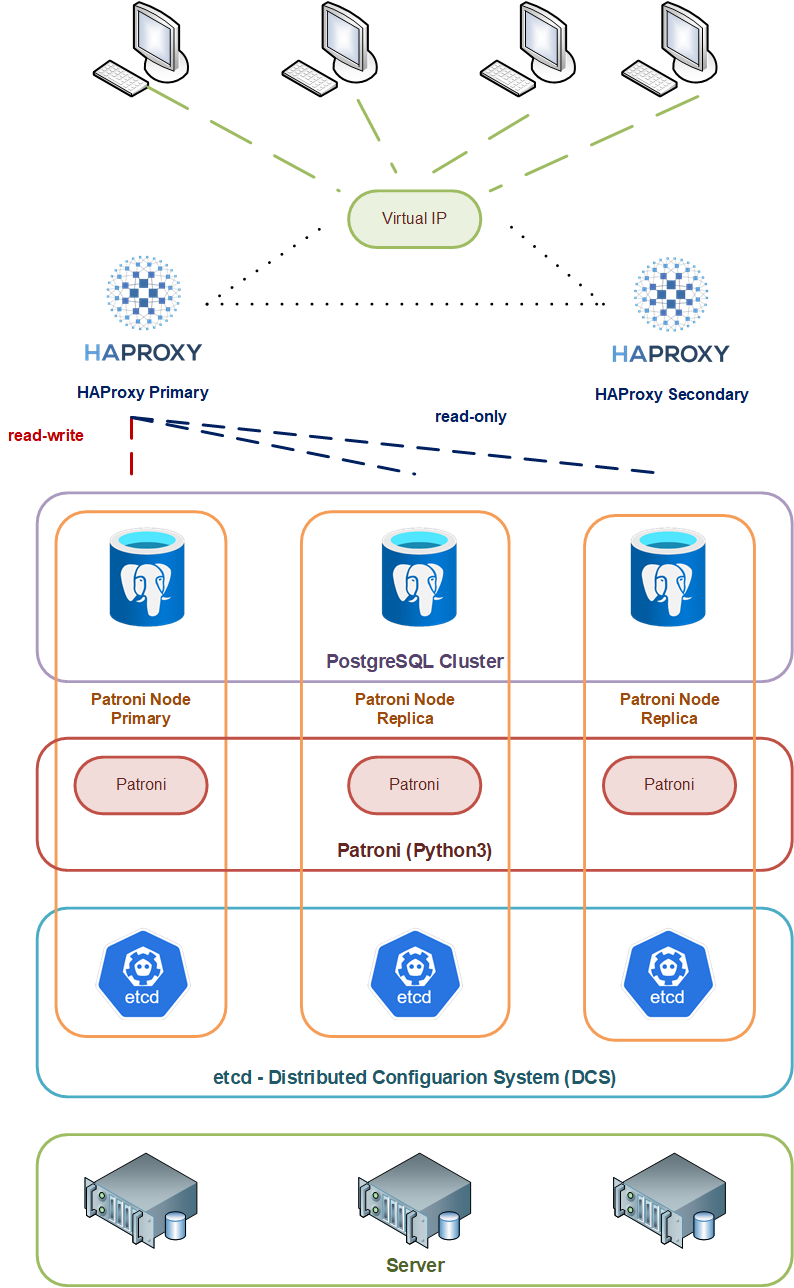
\includegraphics[width=0.75\linewidth]{source/implementation/evaluation/postgresql_ha_solutions/patroni_architecture}
        \caption{Patroni-Architektur}
        \label{fig:patroni-architecture}
    \end{figure}
\end{flushleft}
\begin{flushleft}
    \paragraph{Maintenance}
    Patroni wird von Zalando regelmässig gepflegt.
    Das Projekt hat eine überschaubare Anzahl an Issues, wird aber Regelmässig
    \begin{figure}[H]
        \centering
        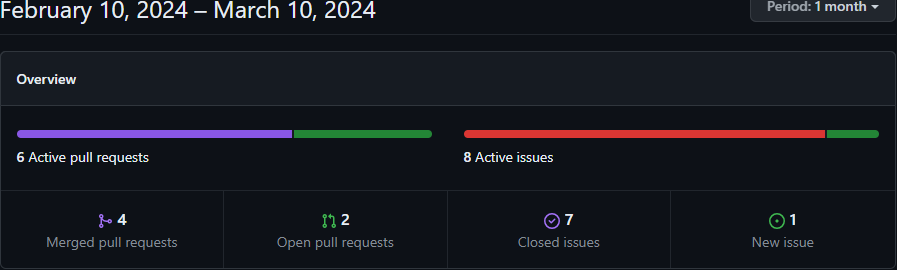
\includegraphics[width=0.75\linewidth]{source/implementation/evaluation/postgresql_ha_solutions/insights/patroni/pulse_zalando_patroni}
        \caption{Patroni - Pulse}
        \label{fig:pulse_zalando_patroni}
    \end{figure}

    Code wird Regelmässig hinzugefügt und entfernt:
    \begin{figure}[H]
        \centering
        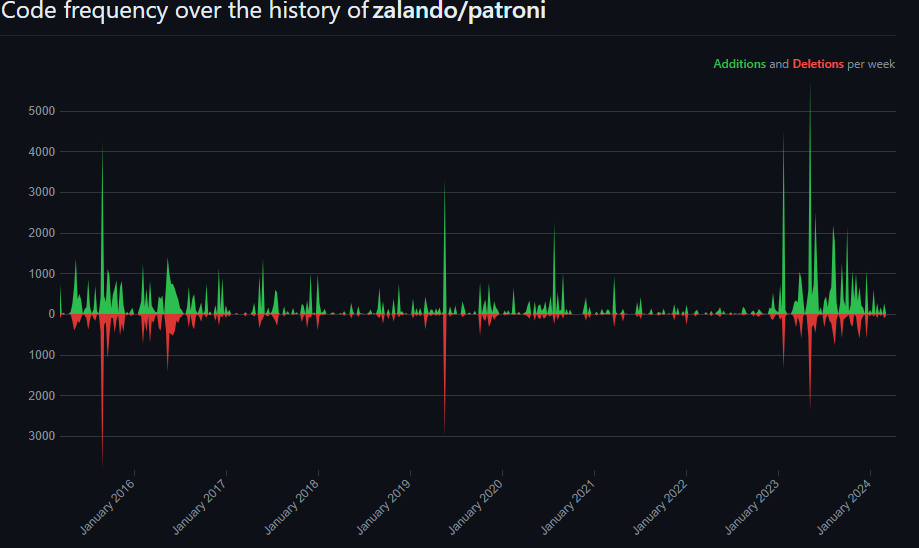
\includegraphics[width=0.75\linewidth]{source/implementation/evaluation/postgresql_ha_solutions/insights/patroni/code_frequency_zalando_patroni}
        \caption{Patroni - Code Frequency}
        \label{fig:code_frequency_zalando_patroni}
    \end{figure}
    Das Projekt hält auch die gängigen Standards auf Github ein:
    \begin{figure}[H]
        \centering
        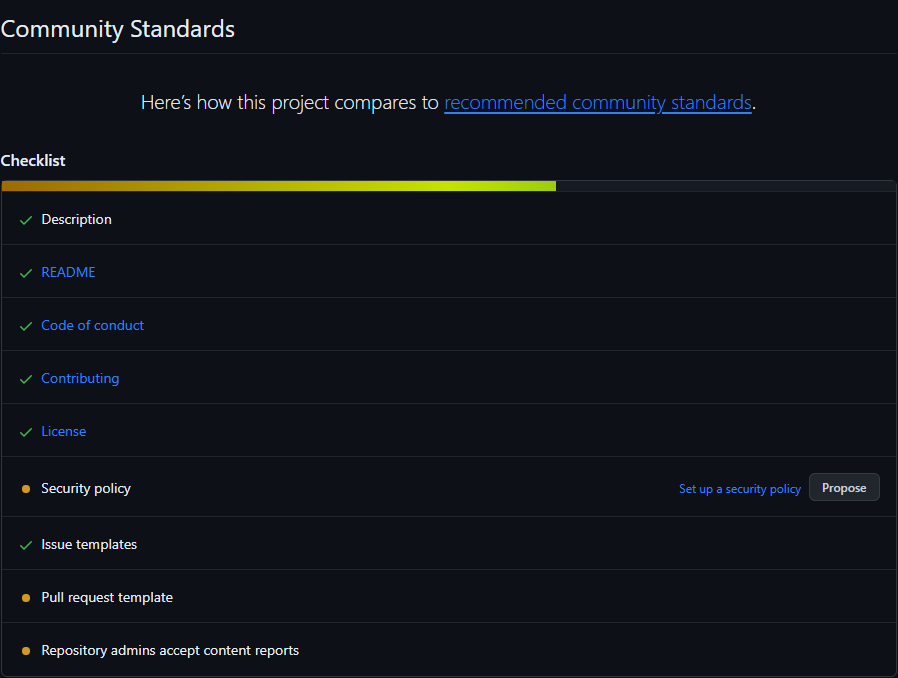
\includegraphics[width=0.75\linewidth]{source/implementation/evaluation/postgresql_ha_solutions/insights/patroni/community_Standards_zalando_patroni}
        \caption{Patroni - Community Standards}
        \label{fig:community_Standards_zalando_patroni}
    \end{figure}

    Die Contributors commiten, löschen und erweitern Patroni Regelmässig:
    \begin{figure}[H]
        \centering
        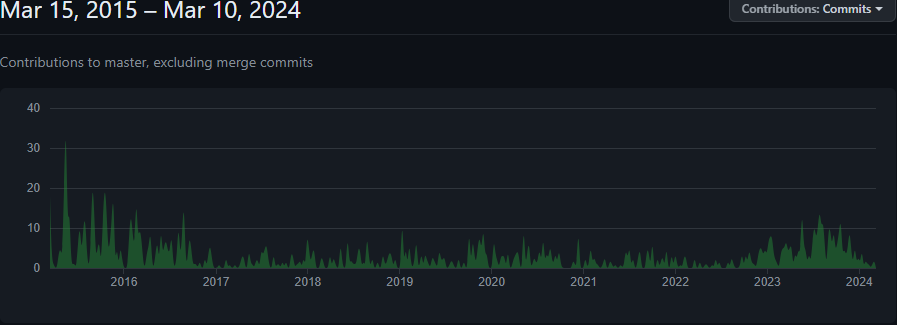
\includegraphics[width=0.75\linewidth]{source/implementation/evaluation/postgresql_ha_solutions/insights/patroni/contributors_commits_zalando_patroni}
        \caption{Patroni - Contributors Commits}
        \label{fig:contributors_commits_zalando_patroni}
    \end{figure}
    \begin{figure}[H]
        \centering
        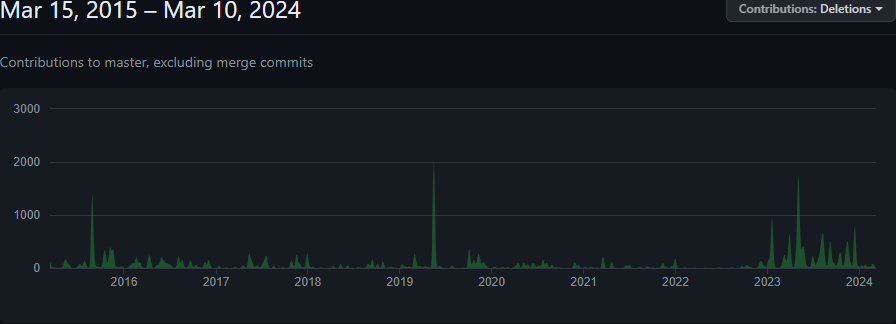
\includegraphics[width=0.75\linewidth]{source/implementation/evaluation/postgresql_ha_solutions/insights/patroni/contributors_deletations_zalando_patroni}
        \caption{Patroni - Contributors Deletations}
        \label{fig:contributors_deletations_zalando_patroni}
    \end{figure}
    \begin{figure}[H]
        \centering
        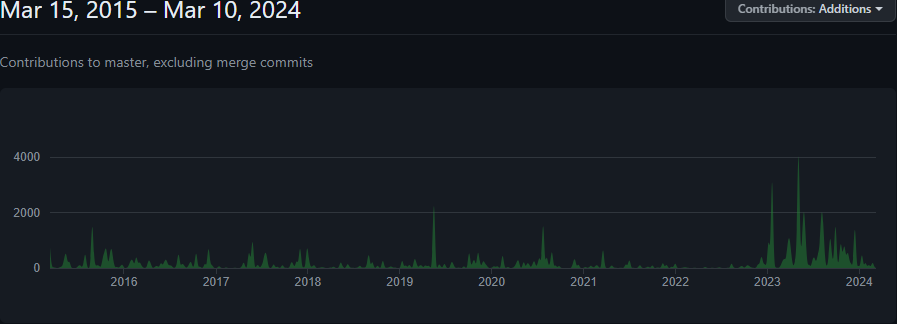
\includegraphics[width=0.75\linewidth]{source/implementation/evaluation/postgresql_ha_solutions/insights/patroni/contributors_additions_zalando_patroni}
        \caption{Patroni - Contributors Additions}
        \label{fig:contributors_additions_zalando_patroni}
    \end{figure}

    Commits werden nach wie vor immer noch Regelmässig eingespielt, auch wenn die Frequenz etwas nachgelassen hat:
    \begin{figure}[H]
        \centering
        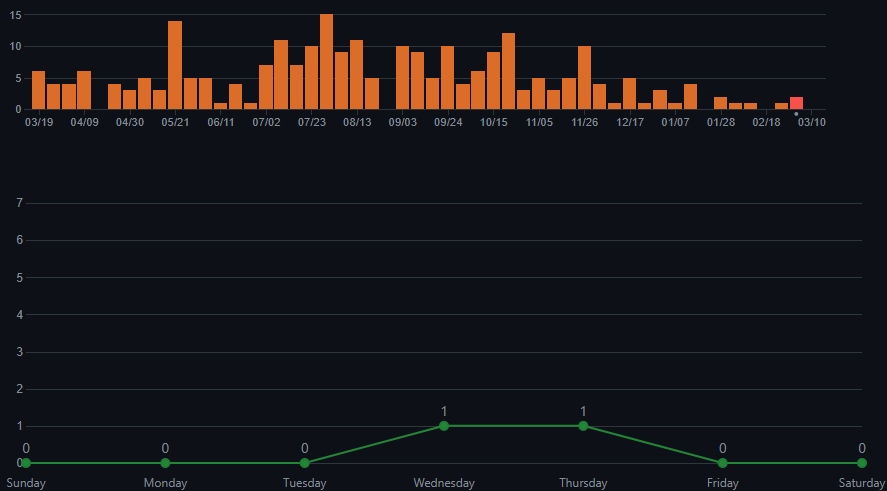
\includegraphics[width=0.75\linewidth]{source/implementation/evaluation/postgresql_ha_solutions/insights/patroni/commit_activity_zalando_patroni}
        \caption{Patroni - Commit Activity}
        \label{fig:commit_activity_zalando_patroni}
    \end{figure}

    Nebst Zalando selbst, hat auch EnterpriseDB\cite{LNF967SI} ein grösseres Repository eingebunden.
    Dies weil EnterpriseDB stark auf Patroni setzt.
     \begin{figure}[H]
        \centering
        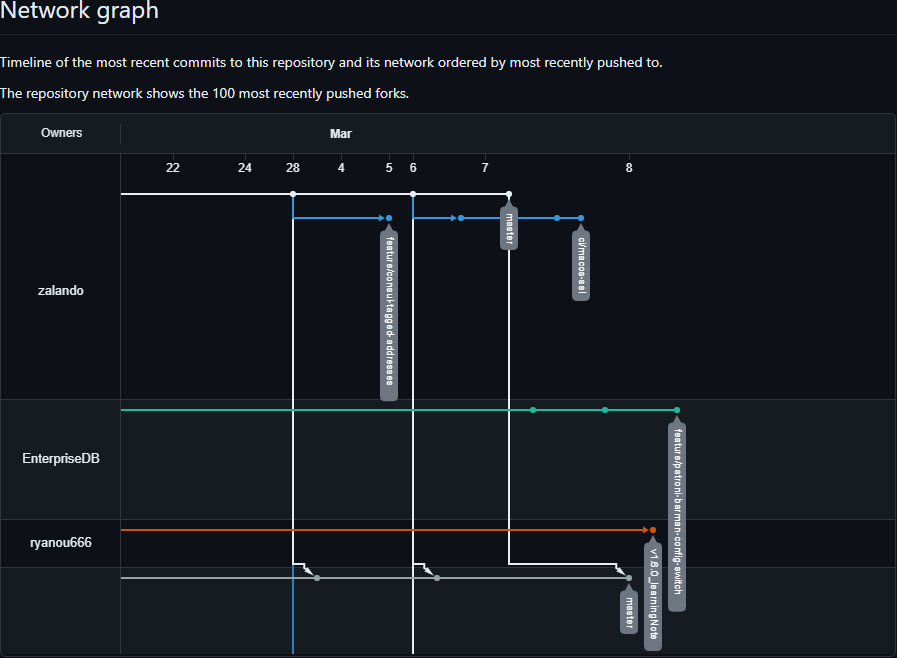
\includegraphics[width=0.75\linewidth]{source/implementation/evaluation/postgresql_ha_solutions/insights/patroni/networkgraph_zalando_patroni}
        \caption{Patroni - Network Graph}
        \label{fig:networkgraph_zalando_patroni}
    \end{figure}
\end{flushleft}